\documentclass[10pt,letterpaper]{article}
\usepackage[top=0.85in,left=2.75in,footskip=0.75in]{geometry}

% Use adjustwidth environment to exceed column width (see example table in text)
\usepackage{changepage}

% Use Unicode characters when possible
\usepackage[utf8]{inputenc}

% textcomp package and marvosym package for additional characters
\usepackage{textcomp,marvosym}

% fixltx2e package for \textsubscript
\usepackage{fixltx2e}

% amsmath and amssymb packages, useful for mathematical formulas and symbols
\usepackage{amsmath,amssymb}

% cite package, to clean up citations in the main text. Do not remove.
\usepackage{cite}

% Use nameref to cite supporting information files (see Supporting Information section for more info)
\usepackage{nameref,hyperref}

% line numbers
\usepackage[right]{lineno}

% ligatures disabled
\usepackage{microtype}
\DisableLigatures[f]{encoding = *, family = * }

% rotating package for sideways tables
\usepackage{rotating}

% Remove comment for double spacing
\usepackage{setspace} 
\doublespacing

% Text layout
\raggedright
\setlength{\parindent}{0.5cm}
\textwidth 5.25in 
\textheight 8.75in

% Bold the 'Figure #' in the caption and separate it from the title/caption with a period
% Captions will be left justified
\usepackage[aboveskip=1pt,labelfont=bf,labelsep=period,justification=raggedright,singlelinecheck=off]{caption}

% Use the PLoS provided BiBTeX style
\bibliographystyle{plos2015}

% Remove brackets from numbering in List of References
\makeatletter
\renewcommand{\@biblabel}[1]{\quad#1.}
\makeatother

% Leave date blank
\date{}

% Header and Footer with logo
\usepackage{lastpage,fancyhdr,graphicx}
\usepackage{epstopdf}
\pagestyle{myheadings}
\pagestyle{fancy}
\fancyhf{}
\lhead{
\includegraphics[width=2.0in]{PLOS-submission.eps}}
\rfoot{\thepage/\pageref{LastPage}}
\renewcommand{\footrule}{\hrule height 2pt \vspace{2mm}}
\fancyheadoffset[L]{2.25in}
\fancyfootoffset[L]{2.25in}
\lfoot{\sf PLOS}

%% Include all macros below

\newcommand{\lorem}{{\bf LOREM}}
\newcommand{\ipsum}{{\bf IPSUM}}

%% END MACROS SECTION


%%% Begin BWP
%\usepackage{amsmath, amsthm, amssymb, wasysym, graphicx}
%\usepackage[small, hang, bf]{caption}
%\usepackage{natbib}
%\renewcommand\cite{\citep}
%\newcommand\citepossessive[1]{\citeauthor{#1}'s \citeyearpar{#1}}
\newcommand\eq[1]{Eq.~\ref{#1}}
\newcommand\fig[1]{Fig.~\ref{#1}}
\newcommand\sref[1]{Section~\ref{#1}}
\let\oldmarginpar\marginpar
\renewcommand{\marginpar}[1]{\oldmarginpar{\linespread{1}\scriptsize{#1}}}

% PLOS wants \paragraph for some reason...
\renewcommand{\subsubsection}[1]{\paragraph{#1}}

\setlength{\marginparwidth}{55mm}


\newcommand\argmin{\mathop{\mbox{{\rm argmin}}}\limits}
\newcommand{\noprint}[1]{}

%%% End BWP


\begin{document}
\vspace*{0.35in}

% Title must be 250 characters or less.
% Please capitalize all terms in the title except conjunctions, prepositions, and articles.
\begin{flushleft}
{\Large
  \textbf\newline{A Multi-Channel Electrode for Chronic Recording and Safe Current-Steered Stimulation}
}
\newline
% Insert author names, affiliations and corresponding author email (do not include titles, positions, or degrees).
\\
Ben Pearre\textsuperscript{1,a,\textcurrency},
Jun S.~Song\textsuperscript{1,c},
Timothy J.~Gardner\textsuperscript{1,d}
\\
\bigskip
\textsuperscript{1} Department of Biology, Boston University, Boston, Massachusetts, United States of America
\\
\bigskip

% Insert additional author notes using the symbols described below. Insert symbol callouts after author names as necessary.
% 
% Remove or comment out the author notes below if they aren't used.
%
% Primary Equal Contribution Note
%\Yinyang These authors contributed equally to this work.
Author \textsuperscript{a}~contributed the original Matlab and LabView implementations and most of the manuscript. Author \textsuperscript{b}~performed the surgeries and histologies.

% Additional Equal Contribution Note
% Also use this double-dagger symbol for special authorship notes, such as senior authorship.
%\ddag These authors also contributed equally to this work.

% Current address notes
%\textcurrency a Insert current address of first author with an address update
% \textcurrency b Insert current address of second author with an address update
% \textcurrency c Insert current address of third author with an address update

% Deceased author note
%\dag Deceased

% Group/Consortium Author Note
%\textpilcrow Membership list can be found in the Acknowledgments section.

% Use the asterisk to denote corresponding authorship and provide email address in note below.
\textsuperscript{\textcurrency} Corresponding author: bwpearre@gmail.com (BP)

\end{flushleft}

\reversemarginpar
%%% End PLOS header template



\begin{abstract}
  Long-term recording enables.... stimulation enables...
  
  Big electrodes --- effective for low-voltage stimulation, but damage going in, gliosis

  Current steering --- dbs: no learning control.  ``Adaptive'' dbs, model-based coarse-grained current steering.
  
  We show that the bundled electrodes splay in the brain.

  We present preliminary results showing that these electrodes can remain capable of recording individual spikes for a year after implantation, even when also used to stimulate.

  We present preliminary evidence that the spatial scale of the splaying is sufficient to allow the steering of current between the electrodes, and that this allows some degree of high-dimensional control over the brain's response to stimulation.
\end{abstract}

\linenumbers

\section{Introduction}



\section{Materials and Methods}




\subsection{Electrode construction}

Electrode arrays were constructed as described in
\cite{Guitchounts2013electrode}.  The charge transfer capacity of one
of the stimulation electrodes was enhanced by electrodeposited iridium
oxide.  \cite{Cogan2008electrodes} describes the electrochemistry of
charge transfer.

\subsubsection{Splay histology}

Electrode bundles were implanted into birds, all to a depth of roughly 3 mm.

The following criteria were used to exclude observations:
\begin{itemize}
\item Electrode shafts lying flat on the surface of the tissue (visible as side-on cylinders).
\item Bundles that were implanted in fibres of passage.
\end{itemize}

\begin{table}
  \begin{tabular}{cccc}
    Good electrodes & Mean dist ($\mu$m) & StdDev dist ($\mu$m) & Max dist ($\mu$m)  \\
    \hline
     3  &  5.0    &    0 &  20.0 \\
   10  &  6.0   & 2.1 &  52.9 \\
   16  &  6.3   & 6.3 &  48.3 \\
    4  &  7.5   & 5.0 &  35.8 \\
    6  & 16.7  & 18.9 &  44.8 \\
    9  &  7.7   & 5.5 & 107 \\
   14 &  12.8  & 12.1 & 15.2 \\
    8 &  14.7  & 17.8 & 108 \\
   15&   15.1  & 10.2 & 163 \\
   15  & 19.3  & 19.1 & 128 \\
    5  & 22.0  & 27.7 & 103 \\
    9  & 28.2   & 35.8 & 148 \\
   11 &  31.8  & 28.1 & 103 \\
    8  & 35.9  & 30.6 & 228 \\
   13 &  76.5 & 152 & 167 \\
    5  & 51.4  & 28.1 &  51.5 \\
    3  & 20.0    &     0 & 123 \\
    6  & 73.5  & 35.5 & 128 \\
    8  & 38.5  & 35.2 & 142 \\
    9  & 47.4  & 31.5 & 208 \\
    5 & 126  & 63.5&  214 \\
    16 &  62.0 &  58.9&  829
  \end{tabular}
  \caption{Raw data.  Each row shows the statistics from one electrode array.  ``Good'' electrodes is the the number of carbon fibre electrodes in each bundle that appeared to still be firmly fixed in the neural tissue after slicing.}
  \label{table:splaydata}
\end{table}

\begin{figure}
  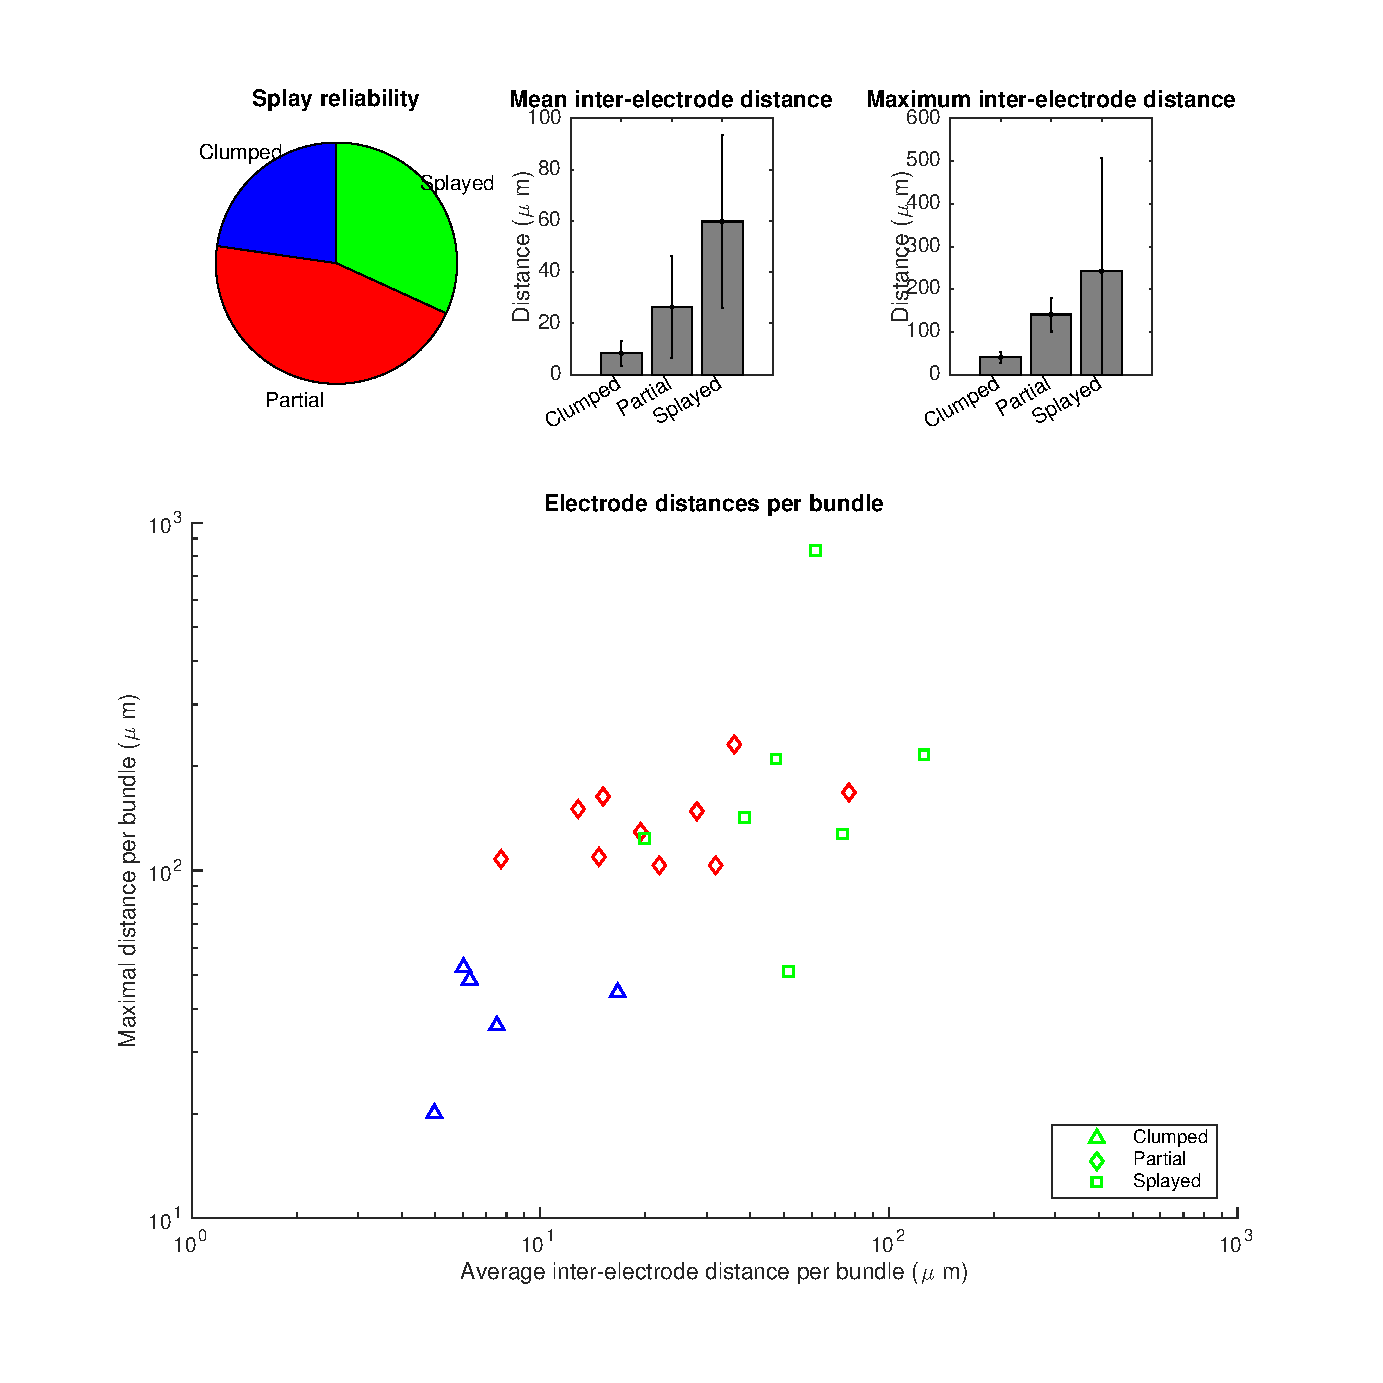
\includegraphics[width=\textwidth]{splay_data}
  \caption{Splay histology data from Table~\ref{table:splaydata}.}
  \label{fig:splaydata}
\end{figure}

After exclusion, 22 arrays, implanted into 13 different birds, yielded at least 3 measurable electrodes.  See Table~\ref{table:data} for the raw data.

\begin{figure}
  % montage -geometry 1024x1024 splay_full.jpeg splay_partial.jpeg splay_no.jpeg splay_montage.eps
  \includegraphics[width=\textwidth]{splay_montage}
  \caption{Splay types, left to right: examples of full splay, partial splay, and no splay.  In all images, black circles are electrode shafts (slices are 50 $\mu m$); in many cases the slicing plane is not quite orthogonal to the electrodes, yielding oblong shapes.  In the bright-field image on the right, three of the electrode slices were pulled out of the tissue during slicing, and appear to lie flat on the slide.  Since their original locations cannot be determined, we have ignored them.}
  \label{fig:splay_montage}
\end{figure}

\begin{figure}
  % montage -geometry 1024x1024 DAPI-and-NeuN*.jpeg damage.eps
  \includegraphics[width=\textwidth]{damage}
  \caption{Damage.  Neural nuclei are shown in green (stained with NeuN) and all cells (e.g. blood) in blue (DAPI).  The presence of non-neural cells indicates damage, and is notable in the vicinity of the largest non-splayed electrode bundle, and nearly absent around individual electrodes.}
  \label{fig:damage}
\end{figure}


\subsection{Zebra finch antidromic HVC $\leftarrow$ X}

\subsection{Recording}

Recordings of spontaneous activity were done using an Intan RHD2000 amplifier at 20 kHz with all possible filtering disabled.

\subsection{Stimulation}

We define stimulation units as follows:

\begin{description}
\item[Channel:] Our electrodes have 16 separate carbon fibres, each one of which we consider a separate channel, since each is connected to a separate amplifier.  Some work better than others, and usually about 75\% of them have low enough impedance to use.  We refer to these as active channels, or just channels.
\item[Pulse:] A biphasic charge-balanced square wave of current.  Each phase is 200 $\mu s$ long, and there is no interpulse interval.
\item[Current-steering configuration (CSC):] The configuration defining which channels receive the positive half of their biphasic pulse first, or vice versa.
\item[Pulse train:] A sequence of 10 identical pulses delivered simultaneously to all active chennels at 25 Hz.  This is slow enough that pulses do not interfere with each other, and is used to detect the reliability of the response.
\item[Threshold scan:] A series of pulse trains, each of which has the same CSC but a different current, designed to find the minimum current for this CSC that will antidromically induce a response in HVC.  The algorithm is described below.
\item[Voltage scan:] The Plexon hardware can deliver a current-controlled pulse to each of 16 channels independently, but only allows one channel at a time to be monitored.  A voltage scan involves sending the same pulse train once per active electrode, monitoring a different one each time.
\end{description}

We used a Plexon stimulator to control stimulation in AreaX, and recorded from HVC using a Tucker-Davis Technologies RZ5 amplifier.  The Plexon self-monitoring channels were recorded on a National Instruments PCI-6251 data acquisition card using the session-based interface of Matlab (various versions from 2014a through 2015b) on Windows 8.1.

We used MATLAB to control the stimulation and acquisition as follows: the National Instruments card is set to record an adequate number of samples of the Plexon self-monitoring channels at 100 kHz, initiated through software, and sending out a TTL pulse at the beginning of acquisition.  The Plexon stimulator begins stimulating upon receipt of that TTL pulse, and the TDT begins recording at 24.414 kHz (the device's native frequency) on the same signal.  Whenever the Plexon is actively delivering current (i.e. during each pulse within the train) it sends out its own TTL pulse: this signal is recorded by the TDT along with the HVC electrode voltages in order to align stimulation pulses with the recording.  The alignment precision is limited only by the sampling rate of the TDT.


\subsubsection{Response detection}

The antidromic response in HVC occurs roughly 3--8 ms after the stimulation pulse, and is highly stereotyped.  In order to detect this reliable response to stimulation, we measure the cross-correlation between the recorded response for each pulse in a train and each other, which provides a robust way of separating neural response from noise.  Because the HVC amplifier's response to the transient stimulation pulse in Area X can persist into the time of interest (3--8 ms), each response is first de-trended using a maximum-likelihood fit over the region 2--25 ms using an eigth order Fourier Series, which removes post-stimulation decay while leaving intact spike-sized signals.  The cross-correlation threshold above which a response is identified is chosen by visual inspection.

As the bird ages, the skull grows down from the implantation site.  For shallow installations such as HVC (depth $\simeq 200\mu m$, the quality of the HVC recordings diminishes as electrodes are forced out of contact with the brain.  This makes it more and more difficult over time to measure the antidromic response.  The above cross-correlation technique is more sensitive than the technique typical of acute or short-term response measurements, in which a pronounced spike is often clearly visible.\marginpar{Need to prevent antidromic response transmission and see if ``measured response'' disappears as it should!  But this requires more birds, and a more complex experiment.} We believe that we are measuring an antidromic response because it is on the correct timescale and appears near the expected stimulation threshold.\marginpar{Cite papers giving timing and stimulation threshold.}


\subsubsection{Threshold scan}



\subsubsection{Voltage scan}


\section{Results}

\subsection{Chronic recording}

\begin{figure}
  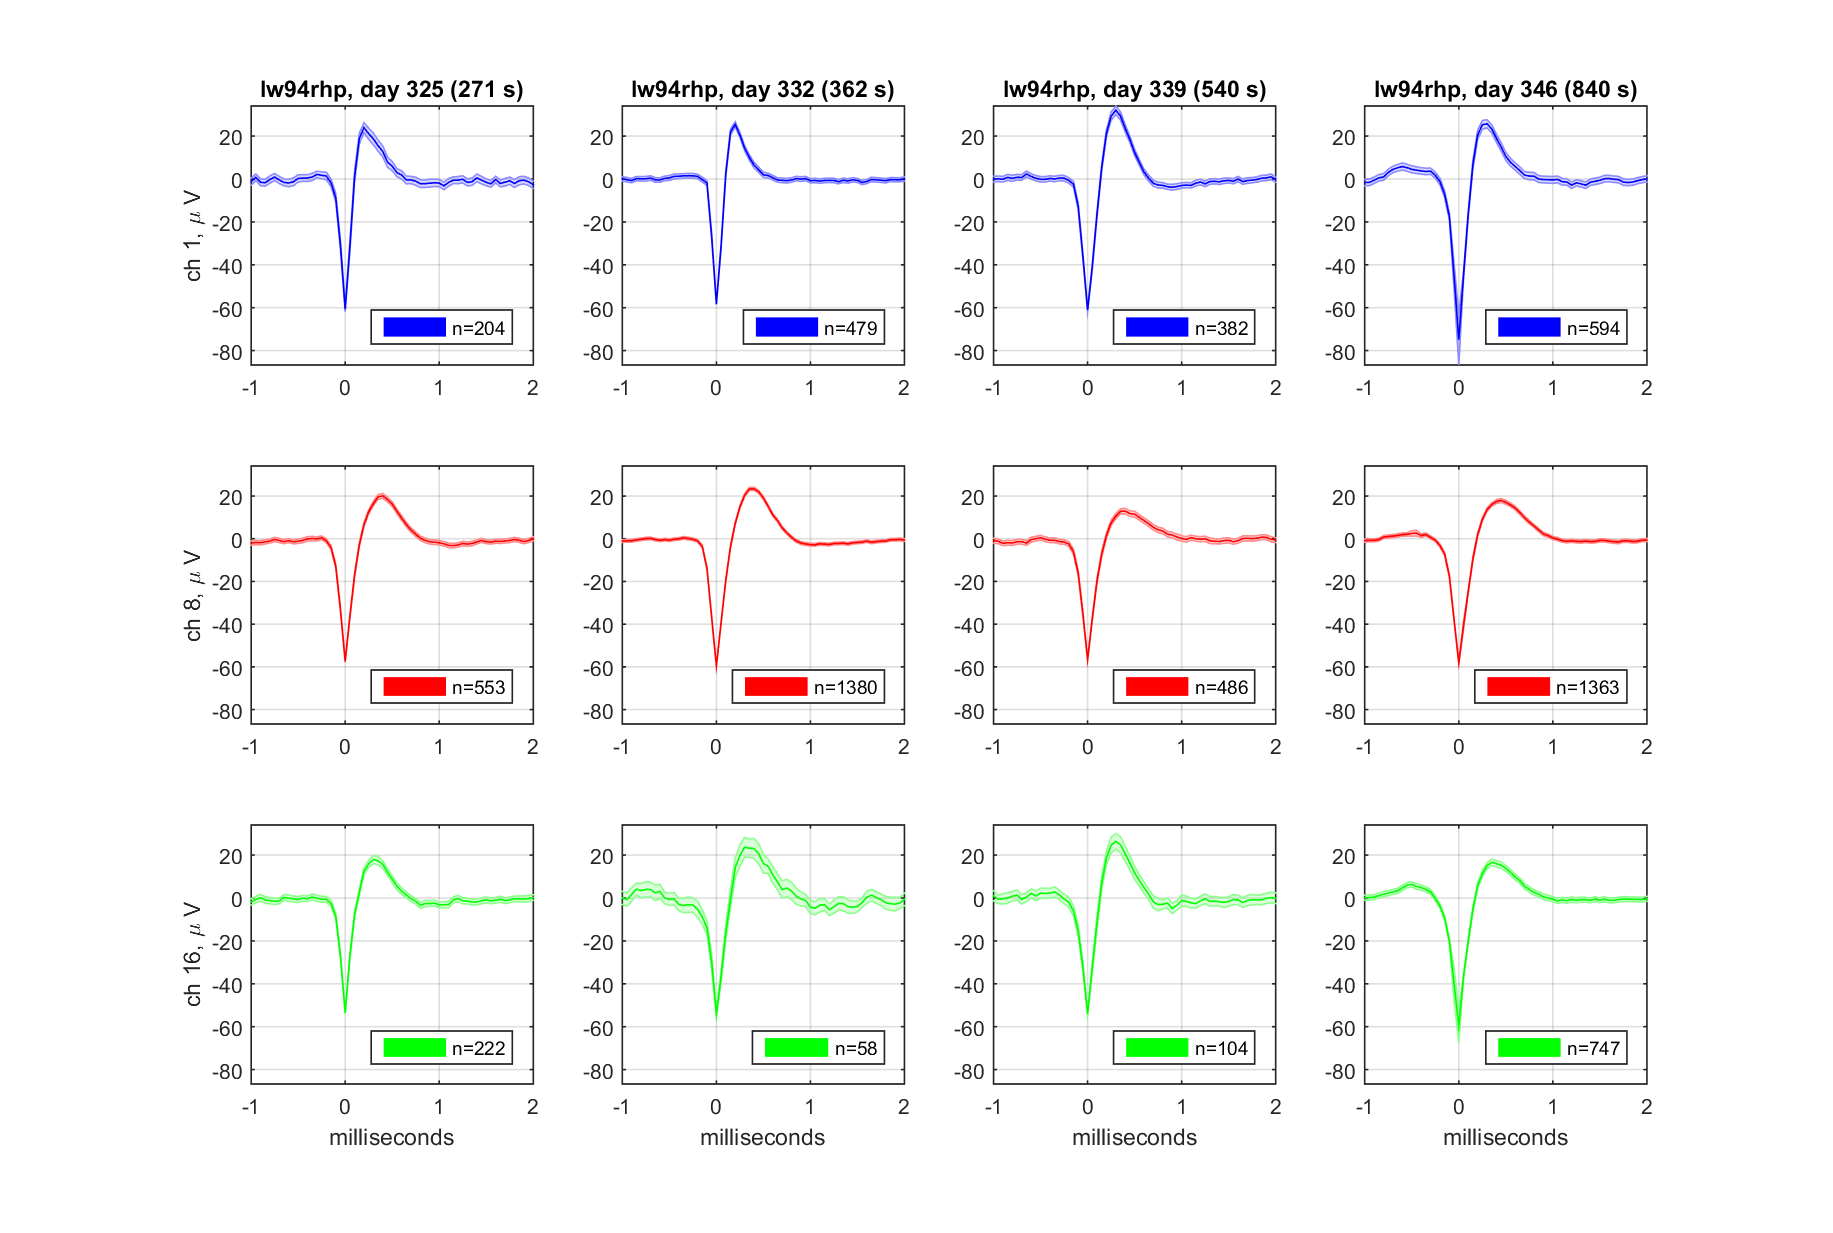
\includegraphics[width=\textwidth]{XSpikeRecording}
  \caption{Some of the electrodes in Area X record spikes after nearly a year.  The column titles show the day post-surgery and the number of seconds of recorded data (for bird lw94rhp).  Each row is one electrode (shown here: only the three best of 16).  Legends show the number of spikes; shaded region is mean $\pm$ 95\% confidence.}
  \label{fig:XSpikeRecording}
\end{figure}


\subsection{Stimulation}

\subsubsection{Minimising stimulation voltage}

\begin{figure}
  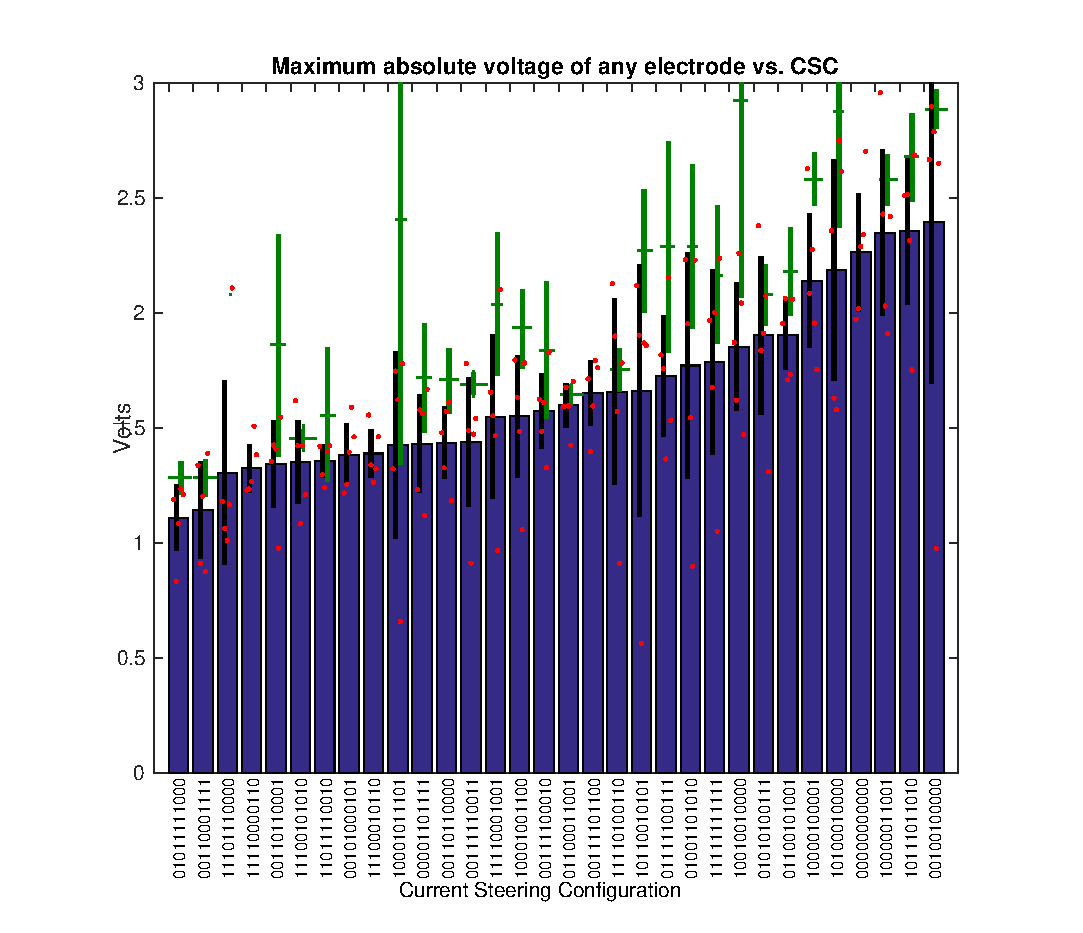
\includegraphics[width=\textwidth]{VoltageVsCSC}
  \caption{The peak X stimulation voltage required in order to achieve biologically effective levels of stimulation in HVC varies with different current-steering configurations.  Here are 32 different configurations, over 5 trials each.  The X axis lists the configuration (each of the 11 active electrodes delivers a positive-first ``0'' or negative-first current-controlled pulse ``1'' pulse).  The Y axis shows the maximum voltage across any electrode.  Error bars are 95\% confidence intervals (n=5), and red dots are the individual trials.  For some CSCs, not all trials evoked a response before our 3V threshold was exceeded, and so the true number is higher.}
  \label{fig:VoltageVsCSC}
\end{figure}

\subsubsection{Controlling the antidromic response}

\begin{figure}
  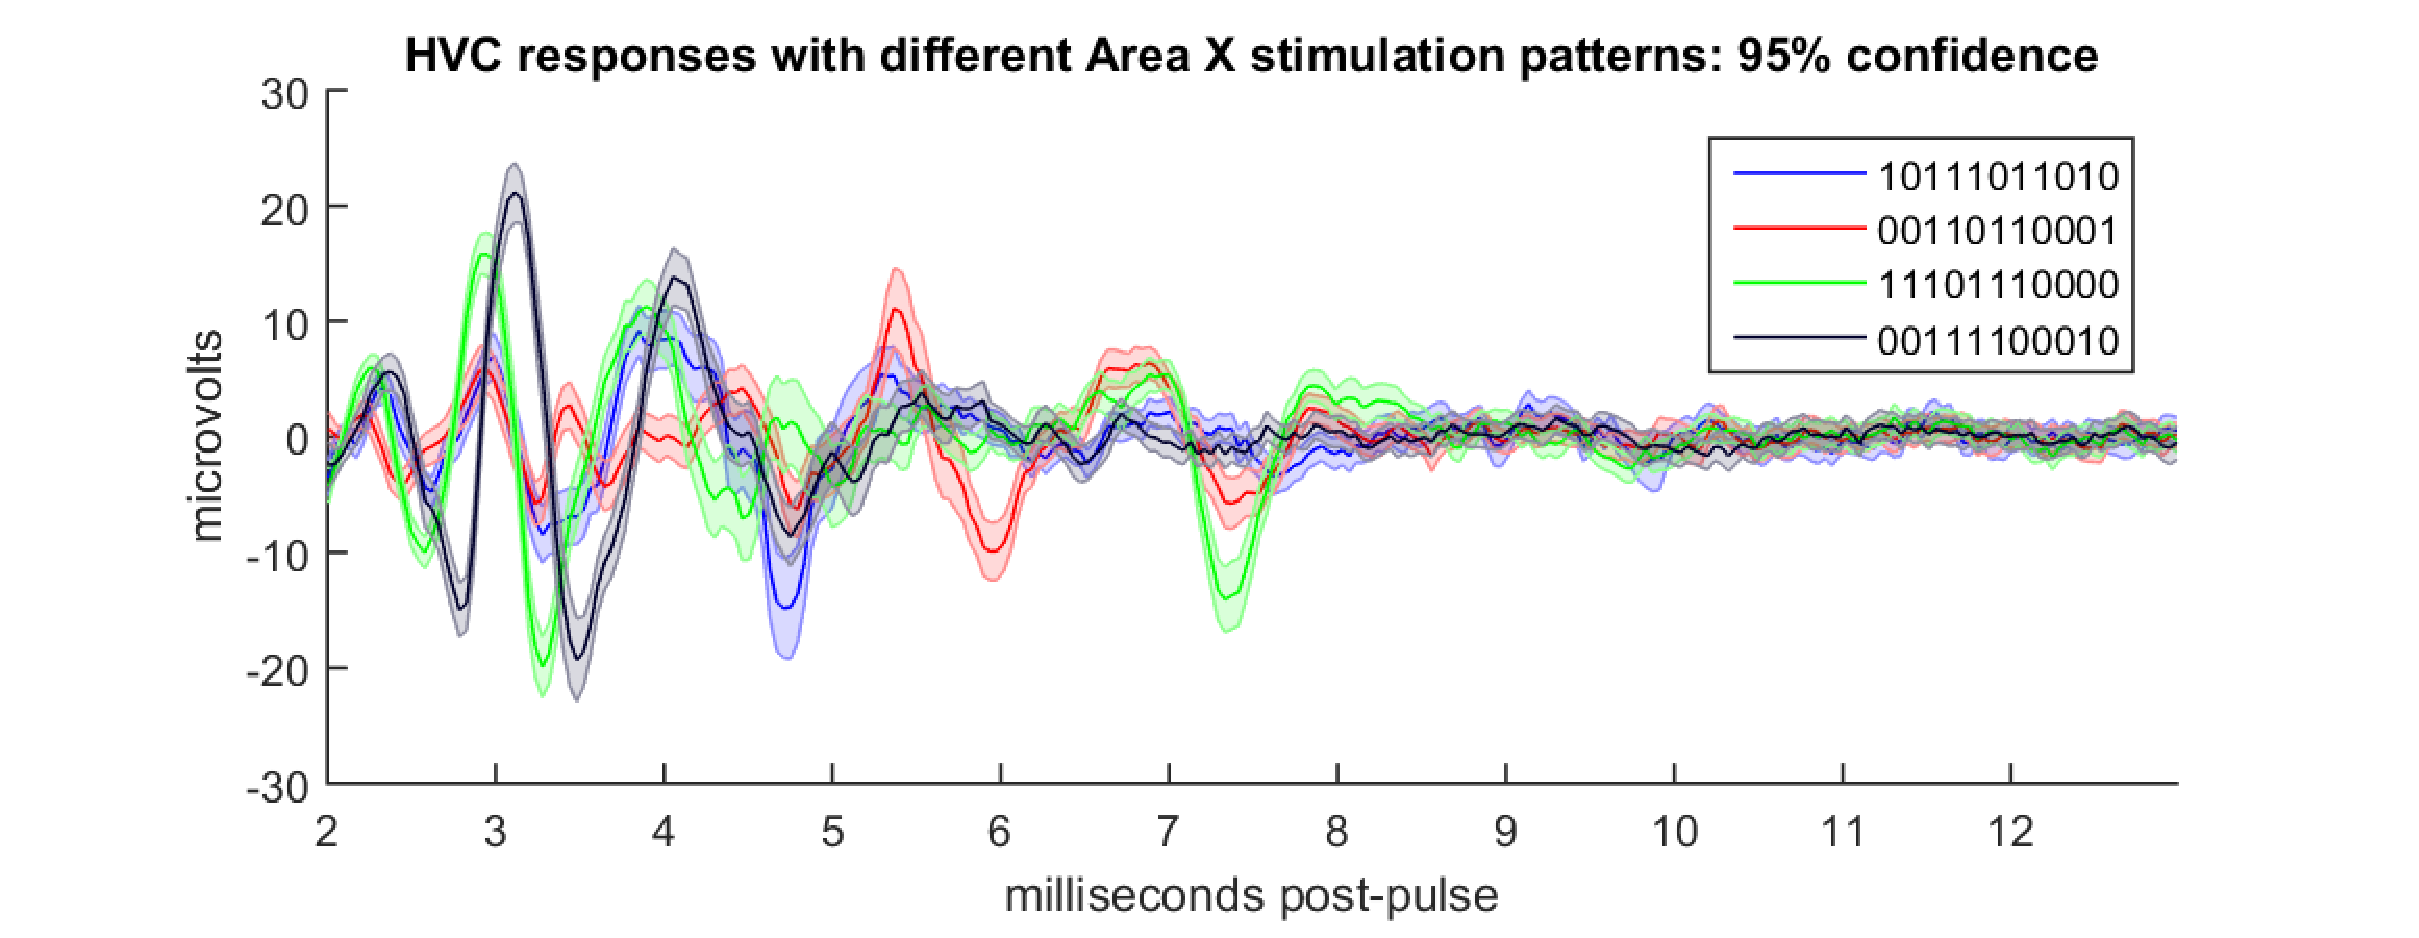
\includegraphics[width=\textwidth]{HVCresponseVsCSC}
  \caption{Different CSCs delivered to Area X can induce different responses antidromically in HVC.  Here are four of the most distinct responses to four of the 32 CSCs shown in \fig{fig:VoltageVsCSC}.  Shading is 95\% confidence, n=198.}
  \label{fig:HVCresponseVsCSC}
\end{figure}


\section{Discussion}

  \cite{Histed2009stimulation}

\bibliography{current}

\end{document}

